\section{Implementation}
\label{sec:implementation}

In this section we describe a prototypical implementation of the previously
described programming model. As a scenario for this, we implement a simple 
online shop.
This scenario enables us to illustrate the concepts described in the foregoing 
chapters of this thesis, as it poses a number of interesting challenges -- such 
as side effects or hidden causalities -- to retroaction.
%
We deliberately do not take functionalities necessary for a productive ``real
world'' online shop into account: authentication, authorization, or validation, 
for example. Considering these features would distract from the concepts which 
we want to illustrate and make the implementation unnecessarily complex. 
Furthermore, we make the assumption that the online shop has only one customer.
This is certainly not realistic, but supporting multiple customers would
merely make the code less clear and comprehensible.
Since we aim for the code and API to illustrate conceptual matters, we thus
deliberately leave out these features and focus on a simple scenario.
%

The prototype was implemented in the scripting language JavaScript, an 
interpreted language with functional aspects. Functions in this language are 
considered higher class citizens and can be used like other variables.
These functional aspects work in favor of our concepts, since they enables us
to e.g. dynamically switch the command processing implementation, supply 
validator functions with retroactive operations, or delay the invocation of 
side effects.
Moreover, JavaScript forms a symbiotic relationship with the lightweight data
format JSON \cite{RFC7159}, which we use in conjunction with the already 
mentioned JSON Patches for the events. 
JSON is also used as the underlying data format when issuing commands and 
queries, or receiving responses.
The prototype was built with node.js\footnote[2]{\href{https://nodejs.org/}{https://nodejs.org/}} 
as the underlying JavaScript platform. Our prototype runs in a single-threaded 
loop, in which incoming commands are processed. 

In the remainder of this chapter we describe further internals of our prototype. 
For this, we focus on the interesting parts and leave some of the underlying 
implementation details (such as persisting events) out.
The code examples are excerpts from our prototypical implementation. In some 
cases we have shortened them to the relevant parts, but they concur with our 
implementation.

\begin{figure}
	\centering
	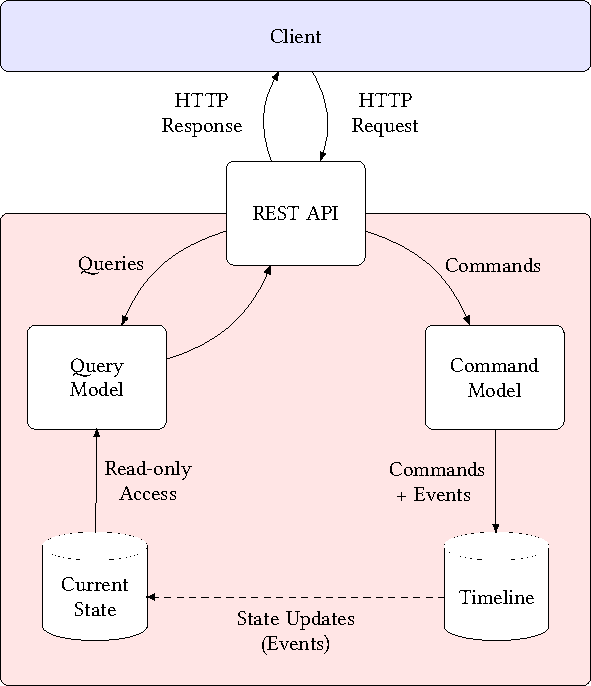
\includegraphics[width=0.5\textwidth]{../illustrations/rest.pdf}
	\caption{
		The figure is a schematic illustration of our prototype.
		A client sends HTTP requests to the REST API and receives a 
		response. The API maps these requests to application commands 
		and queries.
	}
	\label{fig:rest}
\end{figure}

\subsection{The Application Interface}
\begin{table}
\footnotesize
\centering
\begin{tabular}{c | l | l | l | l | l }
 & Semantics 	& Method	 	& Resource	& Payload			& Application Mapping \\
\hline \hline
Q & List all products 		& \cmd{GET} 			& \cmd{/products}	& & \cmd{getProducts()}  				 \\
Q & List details of product 	& \cmd{GET} 			& \cmd{/products/:id}	& & \cmd{getProduct(:id)} 				  \\
 && & & &  \\
Q & Display items in cart 		& \cmd{GET}			& \cmd{/cart}		& & \cmd{getCart()}  				 \\
C & Empty shopping cart 		& \cmd{DELETE}			& \cmd{/cart/}  	& & \cmd{emptyCart()}  \\
C & Put item in cart 		& \cmd{POST}			& \cmd{/cart/:id}	&  \cmd{\{qty: 1\}} & \cmd{addToCart(:id, :qty)} \\
C & Update item quantity  		& \cmd{PUT}			& \cmd{/cart/:id}	&  \cmd{\{qty: 5\}} & \cmd{updateQty(:id, :qty)} \\
C & Remove item from cart 		& \cmd{DELETE}			& \cmd{/cart/:id}	& & \cmd{removeFromCart(:id)} 				  \\
 & & & & \\
C & Place order 			& \cmd{POST}			& \cmd{/order}	& 				& 1) \cmd{fetchCurrencyRate()}  \\
		& & 			& 		& & 2) \cmd{createOrder()} \\
		& & 			& 		& & 2) \cmd{sendConfirmation()} \\
\end{tabular}\\
\caption{The table lists resources and operations of the online shop. 
The REST interface maps and distributes HTTP requests to system commands
(C) and queries (Q). Two application commands yield side effects: 
\cmd{fetchCurrencyRate()} is an external query and returns data,
\cmd{sendConfirmation()} is an external command, which triggers the
transmission of a mail message.
}
\label{tbl:rest-shop}
\end{table}


Representational State Transfer (REST) is a resource-oriented style of architecture~\cite{Fielding2000},
which corresponds to the principles of the World Wide Web. This architectural 
style was introduced by Roy Fielding and has gained popularity in recent years. 
Today, many large web services -- Twitter, Facebook, or Google, for example -- 
utilize REST to provide APIs over the web.
There are numerous reasons for this. Among them is that REST promotes statelessness -- 
each request to an API holds everything needed to fulfill it. The server does not 
hold session state, which makes it easier to build scalable systems.
The most common application of REST is the usage of HTTP to provide web services: 
Uniform Resource Identifiers (URIs) are used as identifiers when accessing 
resources, HTTP methods are used as verbs to operate on these resources. 
The HTTP verbs possess a clearly specified semantics \cite{RFC2616}: 
\texttt{GET} and \texttt{HEAD}, for example, are considered safe and should not 
mutate state, whereas e.g. \texttt{POST}, \texttt{PUT}, or \texttt{DELETE} may 
change state.

Our prototype provides a RESTful API to clients. We chose to use REST, since it 
already provides a clear segregation in queries (safe verbs) and commands (not 
safe verbs). This inherent segregation works in favor of our CQRS architecture. 
The API can be accessed using e.g. a browser or command-line tools, such as cURL 
or wget. 
Table \ref{tbl:rest-shop} lists all resources which are exposed over REST and 
the HTTP verbs which can be used on them. 
%
A shopping cart in a REST architecture is typically modelled as one resource 
\texttt{/cart}, which can be updated using the \texttt{PUT} verb. But in HTTP, 
\texttt{PUT} possesses the semantics of replacing a resource: 
``\emph{The PUT method requests that the enclosed entity be stored under the
supplied Request-URI. [\dots{}] the enclosed entity SHOULD be considered as a 
modified version of the one residing on the origin server.}'' \cite{RFC2616}.
%
This can conflict with retroaction.
As described in Section \ref{sec:command-semantics}, the semantics of commands 
can lead to unintended reversals of retroaction. Here, a \texttt{PUT} command 
overwrites an entire resource each time it is invoked. Thus, retroactively 
injected updates of the cart would be annihilated by the next cart update in 
the timeline.
As a consequence, we modelled individual items in the cart as separate 
resources. By applying \cmd{POST}, items can be added to the cart. Their 
quantity can be updated using \cmd{PUT}.
By applying \cmd{DELETE} on individual cart item resources, they can be removed 
from the cart.

Furthermore, we provide a command with the semantics of emptying the shopping
cart. The operation \texttt{DELETE /cart} can be used to empty the cart. 
This command will annihilate previous \cmd{addToCart()} commands (and events), 
but in this case the semantics is different: delete all items from the cart.
Thus, annihilating prior events is an intended consequence.

In our prototype, HTTP requests are sent to the REST API. This interface 
contains a thin logic layer, it maps and distributes requests to system 
commands and queries.
Figure \ref{fig:rest} depicts a schematic illustration of this process. 
The mapping of application commands and requests is visible in Figure 
\ref{tbl:rest-shop}. In order to fulfill e.g. the \cmd{POST /order} command, 
a \cmd{fetchCurrencyRate()}, a \cmd{CreateOrder()}, and a \cmd{SendConfirmation()} 
command are issued subsequently by the API. 
This is done sequentially; the runtime engine waits for each command to finish 
its execution.
After each command returns, the runtime engine checks if the command succeeded. 
If it did, the command and the resulting event are persisted to the timeline and
the next command in the series is processed. If the command failed, the commands 
in the series will not be processed further. But the commands are still persisted 
to the timeline, in order to enable later replays. 
The following figure depicts a possible course of computation for the mentioned 
series. First, the currency is fetched, then the order creation is attempted. 
This fails and hence the subsequent \cmd{sendConfirmation()} command is not 
processed (highlighted in yellow). It is persisted to the timeline though and 
can be recomputed in a replay.

\begin{figure}[h!]
	\centering
	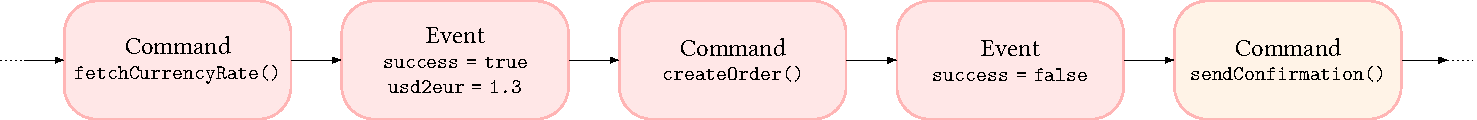
\includegraphics[width=1.0\textwidth]
		{../illustrations/projections3.pdf}

	%\caption{ }
	%\label{fig:projections3}
\end{figure}

Listing \ref{lst:implcp} displays a relevant excerpt from the runtime engine, 
which depicts this process.
The \cmd{fetchCurrencyRate()} has a purely reading side effect (an external 
query). It fetches current currency exchange rates and persists them to the 
system state. These exchange rates are used during the calculation of an order 
price. The \cmd{sendConfirmation()} command triggers a purely writing side 
effect (an external command) which sends irrevocable confirmation messages 
via mail.

\begin{lstlisting}[
	style=styled 
	, caption=Shortened and simplified excerpt from the REST API.
	, label = lst:implcp
]
restAPI.commands = function(request) {
	/* map HTTP requests to commands */
	if (request === "POST /order) {
		var commands = [
			"fetchCurrencyRate(request, state)",
			"createOrder(request, state)",
			"sendConfirmation(request, state)"
		];

		// 1) invoke each command in the series sequentially.
		//    this enforces a causal order by waiting for each 
		//    command to terminate, before the next is invoked.
		// 2) for each comand, calculate event from state changes
		      and persist command + event.
		// 4) publish events to query model(s).
		runtimeEngine.processCommands(commands, request);
	}
}
\end{lstlisting}

\subsection{Command Implementation}
Commands are implemented as modifying the system state object. The runtime 
engine generates an event after a command has been executed. This event
captures the change to the prior state object.
%
Within commands, the programmer annotates which state properties were read 
during the computation. 
Modified state properties are automatically captured by the runtime engine.
This enables the runtime engine to track causalities between events (Section 
\ref{sec:dependent}).
%
Thus, if we e.g. remove a \evt{ProductAddedToCart} event from the timeline, 
subsequent causally dependent events (e.g. \cmd{PlacedOrder}) can be 
automatically removed (or replayed) as well.
Listing \ref{lst:two} depicts two command implementations.

\begin{lstlisting}[
	style=styled, 
	caption={Two examples of online shop commands.},
	label = lst:two
]
/* command, which adds items to the cart */
commands.addToCart = function(request, state){
	/* extract parameters from the HTTP request, update state  */
	var productId = request.params.productId;
	var quantity = request.params.qty;
	state.cart[productId] = quantity;

	return {
		success: true,
		newState: state,
		read: []
	};
}

/* command, which places an order */
commands.placeOrder = function(request, state){
	var order = { items: state.cart, sum: ... }
	state.orders.push(order);
	state.cart = {};

	return {
		success: true,
		newState: state,
		read: []
	};
}
\end{lstlisting}

\subsection{Events}
The already mentioned JSON Patches serve as the data format for events.
Events in our implementation are created automatically by the runtime engine.
We implemented this feature using an open source library\footnote[1]{\href{https://github.com/Starcounter-Jack/JSON-Patch}{https://github.com/Starcounter-Jack/JSON-Patch}},
which offers the possibility to output changes to objects in the form of a 
JSON Patch. For this, it utilizes the \mbox{\texttt{Object.observe()}} feature 
from ECMAScript 2016 (ES7), the most recent specification of the JavaScript 
language. This feature provides a mean for recording changes to an 
object\footnote[2]{\href{https://developer.mozilla.org/de/docs/Web/JavaScript/Reference/Global_Objects/Object/observe}{https://developer.mozilla.org/de/docs/Web/JavaScript/Reference/Global\_Objects/Object/observe}}.
We applied this to record modifications of the system state object.
This enables us to automatically generate the patch after a command has been 
processed. Together with event tags, state properties which were used, and a 
preliminary id (explained later in this section), this patch forms the event.
After the event has been created, it is persisted to the timeline together
with the command. The event is furthermore published to the query model(s).
%
\mbox{Listing \ref{lst:patches}} displays the patches of some events, which were
automatically generated by the prototype runtime engine.

\begin{lstlisting}[
	style = styled, 
	caption = {Events in the form of JSON Patches, from our prototype. They depict modifications of the system state object.},
	label = lst:patches
]
/* add product id 172 to the "state.cart" object with quantity 1 */
[ { "op": "add", "path": "/cart/172", "value": 1 } ]

/* update the quantity of the product "state.cart[172]" */
[ { "op": "replace", "path": "/cart/172", "value": 3 } ]

/* add an object to "state.orders" array and remove it from cart */
[{
	"op": "add",
	"path": "/orders/-",
	"value": {
		"timestamp": 1458061070313,
		"content": { "172": 3 }
	}
}, 
{
	"op": "remove",
	"path": "/cart/172"
}]
\end{lstlisting}

\subsection{Queries}
Queries are sent as HTTP requests to the REST API, using safe HTTP verbs. 
The thin logic layer in the API then maps the requests to a query model, which 
responds with the state visible in the model.
The method in the following listing returns the shopping cart content, when queried.

\begin{lstlisting}[style=styled]
queryModel.getCart = function(request, state) {
	request.send(state.cart);
}
\end{lstlisting}

We apply CQRS here: The query model is decoupled from the command model and 
there might exist a multitude of replicated query model instances which
could be used to conduct e.g. load balancing. 
As examined in Section \ref{sec:cqrs}, this results in an eventually consistent 
behavior of queries.
Listing \ref{lst:rr} displays an excerpt of this routing, using a simple round 
robin algorithm.

\begin{lstlisting}[
	style=styled, 
	caption=Simplified excerpt from the query routing in the API.,
	label= lst:rr
]
restAPI.queries = (request, state) {
	var roundRobin = ++roundRobin % queryModels.length;
	if (request === "GET /cart") {
		queryModel[roundRobin].getCart(request, state));
	}
	// ...
}
\end{lstlisting}

\subsection{Preliminary Command IDs}
\label{sec:prelim}
Following our argumentation from Section \ref{sec:return-values}, we implement 
commands in a way that the HTTP request receives a preliminary command id as an
immediate response. 
This preliminary id can be used by clients to ensure that queries are only 
fulfilled, if the result of a certain command is visible in the query model. 
%
We propose a solution which ties in with the principles behind REST.
Commands in our prototype return the HTTP status code ``\texttt{202 Accepted}'' 
to indicate that the request has been accepted and will be processed
asynchronously. The preliminary id is returned as the payload:

\begin{lstlisting}[style=styled]
HTTP/1.1 202 Accepted 
Content-Type: application/json;charset=utf-8
...

{ "preliminary_id": 533 }
\end{lstlisting}

Queries can be restricted to a certain preliminary id. If this id is not yet 
visible in the query model, the query is rejected. To achieve this, we utilize 
the \texttt{If-Match} field available in HTTP/1.1 as a mean for conditional HTTP 
requests. The specification matches our use case:
``\emph{The 'If-Match' header field makes the request method conditional on
the recipient origin server either having at least one current representation of 
the target resource [\dots{}]}'' \cite{RFC7232}.
%
Listing \ref{lst:testscript} depicts a simple script which we used to test our 
prototype (among other test scripts). The script sends two succeeding HTTP 
requests: a command (line 6-10) and a query (line 14-17). The query is sent as a 
conditional request using the preliminary id which was returned by the prior command.

\pagebreak

\begin{lstlisting}[
	style = styled,
	numbers = left,
	numberstyle = \footnotesize,
	caption = {Simple Test Script for our Prototype.},
	label = lst:testscript
]
#!/bin/ksh
URI=http://localhost:8000

# add item to cart
PRELIMINARY_ID=$(
	curl	-X POST                                     \
		    -H "Content-Type: application/json"         \
		    -d '{ "qty": 3 }'                           \
		    $URI/cart/724                               \
		    | grep -o '[0-9]*'
)

# list items in cart
curl    -v -X GET                                   \
        -H 'Accept: text/plain'                     \
        -H "If-Match: $PRELIMINARY_ID"              \
        $URI/cart
\end{lstlisting}

The command adds a product to the cart and obtains a preliminary id. The HTTP 
exchange looks roughly like in the following listing. Lines starting with 
``\cmd{>}'' indicate a HTTP request from the client to the server, lines 
starting with ``\cmd{<}'' mark the response.

\begin{lstlisting}[style=styled]
> POST /cart/724 HTTP/1.1
> Content-Type: application/json;charset=utf-8
> ...
> 
> { "qty" : 3 }

< HTTP/1.1 202 Accepted 
< Content-Type: application/json;charset=utf-8
< ...
<
< { "preliminary_id": 1458171779004 }
\end{lstlisting}

The second HTTP request (from Listing \ref{lst:testscript}), obtains the content 
of the shopping cart. In accordance to the HTTP/1.1 specification for conditional 
requests, the server returns ``\cmd{304 Not Modified}'' if the condition evaluated 
to false and ``\cmd{200 OK}'' if it succeeded \cite{RFC7232}.
The following listing depicts this rejection (line 5-9) and the alternative response 
(line 13-19).

\begin{lstlisting}[
	style=styled, 
	numbers = left,
	numberstyle = \footnotesize
]
> GET /cart HTTP/1.1
> If-Match: 1458171779004
> ...

< HTTP/1.1 304 Not modified
< Content-Type: application/json;charset=utf-8
< ...
<
< { "visible" : false }

OR

< HTTP/1.1 200 OK
< Content-Type: application/json;charset=utf-8
< ...
<
< [ 
< 	{ "product1" : { "title": "Lorem Ipsum", "price": 99 }  }
< ]
\end{lstlisting}


\subsection{Retroactive Use Cases}
In this section we describe some of the use cases for retroaction, which 
can be applied to our prototype. %which we implemented in the prototype.

\subsubsection{History-aware Algorithms}
Through the programming model which we described, the history of the application 
is exposed to commands. This can be utilized to create history-aware algorithms.
An example for this is a \cmd{PlaceOrder} command which calculates an order 
discount based on previous orders by this customer. Listing \ref{lst:impl-po1}
depicts the commands' implementation.
First, a branch of the timeline is created, then all events tagged with 
\evt{placed-order} are searched for. Next, these events are examined in order 
to compute a discount for the current order.

\begin{lstlisting}[
	  style = styled 
	, caption = {When placing an order, a discount based on previous orders is calculated.}
	, label = lst:impl-po1
]
commands.placeOrder = function(request, state) {
	/* 'big bang' is a pre-defined tag of the runtime engine which
	   refers to the start of the timeline. */
	var b = retroactive.createBranch("big bang");

	/* find all events tagged with 'placed-order' */
	var orderEvents = b.getEvents(["placed-order"]);

	var allOrdersAmount = 0;
	for (var o in orderEvents) {
		/* get the system state object at the point of this event 
		   in the timeline */
		allOrdersAmount += orderEvents[o].getState().totalAmount;
	}

	var discount = 0;
	if (allOrdersAmount > 1000) discount = 0.1;      /* 10% */
	else if (allOrdersAmount > 100) discount = 0.05; /*  5% */

	var order = {
		items: ...,
		totalAmount: ... * discount
	};
	state.orders.push(order);

	return { success: ..., newState: ..., read: ... };
}
\end{lstlisting}


\subsubsection{Partial Replay with Control of Side Effects}
The concept of partial replays allows for control of the side effects in a 
replay (Section \ref{sec:replaying-se}).
It is possible to either reuse prior results or reinvoke them and continue 
the processing with these new results. As we described it, the shop fetches 
current currency exchange rates before creating an order. A use case is to 
replay the shop timeline and reprocess each \cmd{fetchCurrencyRate()}.
In such a replay, the shop fetches each currency exchange rate from an 
external web service again. Each causally dependent command (\cmd{placeOrder()} 
in this case) will then be reprocessed with the new result.
In order to prevent confirmations from being sent out again, we suppress them.
In this case, suppressing the invocation means that we reuse the event from the 
last \cmd{sendConfirmation()} invocation (if an event is available).

\begin{lstlisting}[
	  style = styled 
	, caption = {Partial Replay Example}
	, label = lst:impl-po2
]
/* newly compute the events in this array, instead of reusing the 
   already persisted ones */
var recomputeCommands = [ "fetch-currency-rate" ];

/* for the tags in the array use the persisted events instead of 
   newly invoking the command */
var reuseEvents= [ "confirmation-mail" ];

/* normal event replay, but for the supplied 'newlyComputeEvents'
   array the belonging command is newly invoked. Events which
   possess a causal relationship to the newly computed ones are
   recomputed as well, as long as they are not specified in the
   'reuseEvents' array. */
var b = createBranch("big bang");
b.partialReplay({ recompute: recomputeCommands, reuse: reuseEvents });
\end{lstlisting}

In the code above \emph{all} \cmd{fetchCurrencyRate()} commands and the direct 
and indirect causally related events are reprocessed. 
But it would also have been possible to reprocess just a single specific 
\cmd{fetchCurrencyRate()} and its causally related events. 
This can be achieved through the usage of unique (or appropriately fine-grained)
tags within the commands. These tags can then be filtered for in a later replay.

\subsubsection{Alternate Command Behavior}
We can adapt the above code to evaluate how different currency exchange rates
would have affected the state. 
To achieve this, we exchange the \cmd{fetchCurrencyRate()} command in a branch. 
Instead a function which returns hypothetical exchange rates from a fixed list
is used. Then a replay of the relevant commands is conducted. Next, the resulting 
state can be accessed for further analysis:

\begin{lstlisting}[style=styled]
var experimentalRatesFn = function(request, state) {
	/* use this fixed currency rate for the new processing */
	state.currencyRates = { eur2usd: 1.13 };

	return { 
		success: true, 
		newState: state, 
		read: [] 
	};
}

var someCommand = function(request, state) {
	b.createBranch("big bang");
	b.changeCommandFunction("fetchCurrencyRate", 
	                        "experimentalRatesFn");
	
	b.partialReplay({ 
		recompute: ["fetch-currency"],
		reuse: ["confirmation-mail"]
	});

	var experimentalOrders = b.getState().orders;

	// further processing
	// ...

	return { success: true, newState: ..., read: ... };
}
\end{lstlisting}

\subsubsection{Observe Alternate States}
We implemented a feature which allows for displaying how the orders would have 
been different, if customers would not have removed any products from their cart.
For this, a branch is created and all events tagged with \evt{product-removed-from-cart} 
are deleted from it. Next, a replay of commands tagged with \cmd{place-order} 
is conducted.

\begin{lstlisting}[style=styled]
commands.calculatePossibleOrders = function(request, state) {
	var b = retroactive.createBranch("big bang");

	/* supplying true would remove all causally dependent 
	   "place-order" events as well. */
	b.deleteEvents("product-removed-from-cart", false);

	/* only these commands (and the ones which read state modified 
	   by these ones) are recomputed, for other commands the events 
	   are reused */
	var recomputeCommands = [ "place-order" ];

	var b = createBranch("big bang");
	var reuseEvents = ["confirmation-mail"];
	b.partialReplay({ 
		recompute: recomputeCommands, 
		reuse: reuseEvents 
	});

	var branchState = b.getState();
	state.whatifOrders = branchState.orders;

	return {
		newState: state,
		success: true,
		read: []
	};
}
\end{lstlisting}

The result from this analysis is saved to the state property \cmd{state.whatifOrders} 
and subsequently persisted to the timeline as an event, by the runtime engine.
The query model(s) eventually receive the events as state updates. Then the 
results are visible in the query model. They are exposed to the clients through 
a query:

\begin{lstlisting}[style=styled]
queries.getPossibleOrders = function(request, state) {
	return state.whatifOrders;
}
\end{lstlisting}

\subsubsection{Retroaction for Optimization}
It is possible to use the application's history for optimization or adaption of
the application's current behavior. This is the use case which we described in 
Chapter \ref{chp:related-work} as history-aware and self-improving algorithms.
%
Concerning the online shop, this section described the implementation of a 
history-aware discount algorithm. But it is also possible to use the system's 
history for evaluating experimental -- and possibly better performing -- 
algorithms. This can be achieved by replaying commands from the timeline
with a different command processing implementation. The resulting state can 
then be used for comparison against the current state of the timeline -- and 
thus against the current discount algorithm. 
Next, we can adapt the future application behavior based on these insights.

To achieve this, we create a command which creates a branch, exchanges the 
\mbox{\cmd{placeOrder()}} command implementation, conducts a replay, and 
compares the branch state against the application state. Based on this result, 
the current command function can then be exchanged.

\begin{lstlisting}[style=styled]
commands.tags.placeOrder = ["place-order"];
commands.experimentalFn = function(request, state) { ... }

commands.optimizeAlgorithm = function(request, state) {
	var b = createBranch("beginning of timeline");
	b.changeCommandFunction("placeOrder", "experimentalFn");
	b.partialReplay({ recompute: [ "place-order" ] });

	/* compare branch state against current state */
	var branchState = b.getState();
	if (...) {
		/* exchange command function in ongoing timeline */
		changeCommandFunction("commands.placeOrder", 
                          "commands.experimentalFn");
	}

	return ...;
}
\end{lstlisting}

In order to compare different processing implementations against each other,
it has to be clear that the differences after a replay have occurred due to
the different command processing implementation. 
Therefore a deterministic command replay needs to be ensured. If commands are 
processed in a different order, the differences might as well be due to this 
indeterminism. Hidden causalities need to be taken into account as well, 
otherwise one could mistakenly attribute differences in the outcome to the 
different command processing, although hidden causalities or side effects 
could be responsible as well.

\subsubsection{Iterate Towards Target State}
A further use case is to define a target state and modify the past until we 
reach it. We can determine if we get from a specified start state to a defined 
target state by applying subsequent, iterative modifications.
This feature is especially interesting for problems where modifications have 
to be ``played through'' and cannot be trivially calculated. 
%
For example, the online shop could have a complex algorithm, which calculates
price increases each time an order is placed.
Lets say this calculation is complex. It depends on the state of the system at 
the time when an order is placed and takes the number of similar recent product 
orders into account. 
If we want to find out how much more orders would have had to be placed for
the current price of a product to reach a specified state, we can retroactively
insert orders until we reach our target state.

But this strategy is not limited to insertion or removal operations of commands 
and events. It can also be applied to the command processing implementation, to 
determine how the logic needs to be modified to reach a certain state. This 
process then yields the necessary modifications.
In general, this can be beneficial for a lot more cases, where the behavior of 
the application over time needs to be considered or is time-dependent.
We imagine that this feature allows for novel debugging schemes and bug fixes. 

\subsection{Prototype Limitations}
A limitation of our prototype is that if one command in the series fails, the 
series will not be executed further. This limits the expressiveness, since 
rollbacks of commands in the series are not possible.
Additionally, it is not possible to issue a hierarchical series, where parts of
the series can be executed independent of each other. 

The annotation, which state properties were used for the computation of a
state change, is cumbersome and could probably be done by an underlying 
runtime engine. We are confident that this could be achieved through source 
code analysis, by observing which state properties are accessed and modified.
Another option is to use explicit getter and setter methods when accessing 
properties of the state object.
Such methods can record the access of state properties as well.

Last, we have by far not exhausted the possibilities for retroactive operations,
which the API could expose. For example, forward deleting all events from a certain
branching point could be helpful, if the objective is to append simulated
events from a certain point on. This is not possible with our described
prototype, but could certainly be implemented. We have restrained our description
to a basic set of operations to keep the concept simple and comprehensible.
